\documentclass[handout,compress]{beamer}

\usetheme[block=fill]{metropolis}

\usepackage{graphicx} % Allows including images
\usepackage{amsmath,amsfonts,amsthm,amssymb}
\usepackage{color}
\usepackage{xcolor,cancel}
%\setitemize{label=\usebeamerfont*{itemize item}%
%	\usebeamercolor[fg]{itemize item}
%	\usebeamertemplate{itemize item}}
\definecolor{mDarkBrown}{HTML}{604c38}
\definecolor{mDarkTeal}{HTML}{23373b}
\definecolor{mLightBrown}{HTML}{EB811B}
\definecolor{mMediumBrown}{HTML}{C87A2F}
\definecolor{mygreen}{HTML}{98C2B9}
\definecolor{myyellow}{HTML}{DFD79C}
\definecolor{myblue}{HTML}{8CA7CC}
\definecolor{kern}{HTML}{8CC2B7}

\usepackage{float}
\usepackage{framed}
\usepackage{epsfig}
\usepackage{graphicx}
\usepackage{subcaption}
\usepackage{ulem}
\usepackage{hhline}
\usepackage{multirow}
\usepackage{comment}   
\usepackage{bbm}
\usepackage{tikz}   
\usepackage{ulem}
\def\Put(#1,#2)#3{\leavevmode\makebox(0,0){\put(#1,#2){#3}}}
\newcommand*\mystrut[1]{\vrule width0pt height0pt depth#1\relax}
\newcommand{\eqdef}{\mathbin{\stackrel{\rm def}{=}}}


\newcommand{\bs}[1]{\boldsymbol{#1}}
\newcommand{\bv}[1]{\mathbf{#1}}
\newcommand{\R}{\mathbb{R}}
\newcommand{\E}{\mathbb{E}}

\DeclareMathOperator*{\argmin}{arg\,min}
\DeclareMathOperator*{\argmax}{arg\,max}
\DeclareMathOperator{\nnz}{nnz}
\DeclareMathOperator{\Var}{Var}
\DeclareMathOperator{\sinc}{sinc}
\DeclareMathOperator{\mv}{mv}
\DeclareMathOperator{\sgn}{sgn}
\DeclareMathOperator{\step}{step}
\DeclareMathOperator{\gap}{gap}
\DeclareMathOperator{\poly}{poly}
\DeclareMathOperator{\tr}{tr}
\DeclareMathOperator{\orth}{orth}
\newcommand{\norm}[1]{\|#1\|}
\captionsetup[subfigure]{labelformat=empty}
\captionsetup[figure]{labelformat=empty}
\DeclareMathOperator*{\lmin}{\lambda_{min}}
\DeclareMathOperator*{\lmax}{\lambda_{max}}

\newcommand{\specialcell}[2][c]{%
  \begin{tabular}[#1]{@{}c@{}}#2\end{tabular}}
\newcommand{\specialcellleft}[2][c]{%
\begin{tabular}[#1]{@{}l@{}}#2\end{tabular}
}

\usepackage{tabstackengine}
\stackMath


%----------------------------------------------------------------------------------------
%	TITLE PAGE
%----------------------------------------------------------------------------------------

\title{CS-UY 4563: Lecture 8 \\ Finishing the Bayesian Perspective, Linear Classifiers}
\author{NYU Tandon School of Engineering, Prof. Christopher Musco}
\date{}

\begin{document}

\begin{frame}
	\titlepage 
\end{frame}

\metroset{titleformat=smallcaps}

\begin{comment}
\end{comment}

\begin{frame}
	\frametitle{probabilistic modeling}
	\emph{Bayesian} or \emph{Probabilistic} approach to machine learning:
	\begin{itemize}
		\item Decide on simple probabilistic model with parameters $\vec{\theta}$ which could explain our data $(\vec{x}_1, y_1), \ldots, (\vec{x}_n, y_n)$. 
		\item Learn $\vec{\theta}$ from past data. 
		\item Given a new input $\vec{x}$, predict $y$ (either a class label or regression value) using the probabilistic model.
	\end{itemize}
\begin{center}
	Typically prediction $y$ is chosen to be the \textbf{maximum a posterior (MAP) estimate} under the assumption that data comes from our chosen probabilistic model.
\end{center}
\end{frame}



\begin{frame}
	\frametitle{naive bayes classifier}
	\textbf{Example from last class:}
	\begin{itemize}
		\item Given binary inputs $(\vec{x}_1, y_1), \ldots, (\vec{x}_n, y_n)$ (e.g. email bag-of-words vectors and binary labels)
		\item Came up with model for how $\vec{x}_i,y_i$ might be generated.
		\item Computed MAP estimate using Bayes rule.
	\end{itemize}
\begin{center}
	This gave us the \textbf{\alert{Naive Bayes Classifier}}.
\end{center}
\end{frame}

\begin{frame}[standout]
	other applications of \\
	\alert{the bayesian perspective}
\end{frame}

\begin{frame}
	\frametitle{bayesian regression}
	The Bayesian view offers an interesting alternative perspective on \emph{many} machine learning techniques. 
	
	\vspace{1em}
	\textbf{Example:} Linear Regression. 
	
	\textbf{Probabilistic model:}
	\begin{align*}
	 	y_i = \langle \vec{x}_i, \vec{\beta} \rangle+ \eta
	\end{align*}
	where $\eta$ is a \textbf{Gaussian random variable} with variance $\sigma^2$.
	
	(Here we assume $\vec{x}_1, \ldots, \vec{x}_n$ are \textbf{fixed}, not random. This is called a ``fixed design" setting.)
	\vspace{.5em}
	\begin{columns}
		\begin{column}{.5\textwidth}
				\hspace{2em}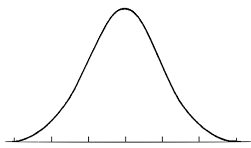
\includegraphics[width=.7\textwidth]{bell.png}
		\end{column}
		\begin{column}{.5\textwidth}
				$Pr(\eta = z) \sim \frac{1}{\sqrt{2\pi\sigma^2}} e^{-z^2/\sigma^2}$
		\end{column}
	\end{columns}
\end{frame}

\begin{frame}
	\frametitle{bayesian regression}
	Not a perfect model, but simple and reasonable:
	\begin{center}
		\includegraphics[width=.45\textwidth]{real_data.png} \includegraphics[width=.45\textwidth]{modeled_data.png}
		
		\small{To make the plot on right I used numpy's \texttt{random} library and the \texttt{randn} function for generating Gaussian (normal) random numbers:
			
		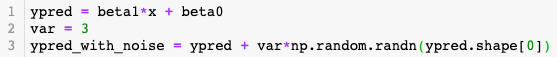
\includegraphics[width=.9\textwidth]{randn.png}}
	\end{center}
	
\end{frame}

\begin{frame}
	\frametitle{quick check}
	\textbf{Example:} Linear Regression. 

	\textbf{Probabilistic model:}
	\begin{align*}
	y_i = \langle \vec{x}_i, \vec{\beta} \rangle+ \eta
	\end{align*}	
	where $\eta$ is a \textbf{Gaussian random variable} with variance $\sigma^2$.
	
	
	\begin{center}
		Suppose we learn $\vec{\beta}$ using past data. What is the \emph{maximum a posterior (MAP)} estimate $y^*$ given observed data $\vec{x}$?
	\end{center}

\begin{itemize}
	\item Want to find $y^*$ which maximizes $\max_{y} \Pr(y \mid \vec{x})$. 
	\item Under our model, $y = \langle \vec{x}, \vec{\beta} \rangle+ \eta$.
	\item So $\Pr(y \mid \vec{x})$ is equal to $\Pr(\eta = y - \langle \vec{x}, \vec{\beta} \rangle)$
	\item $\Pr(\eta = y - \langle \vec{x}, \vec{\beta} \rangle)$ is maximized at $y - \langle \vec{x}, \vec{\beta} \rangle = 0$.
	\item So $y^* = \langle \vec{x}, \vec{\beta} \rangle$ is the MAP estimate.
\end{itemize}
\end{frame}

\begin{frame}
	\frametitle{bayesian regression}
	\begin{center}
		\alert{How should we learn $\vec{\beta}$ for our model from prior data?}
	\end{center}
		\textbf{Bayesian approach:} Use MAP estimate again! But this time for the parameter vector itself, not just for prediction.
		
		 Give data matrix $\bv{X}\in \R^{n\times d}$ and target vector $\vec{y} \in \R^n$, choose $\vec{\beta}^*$ to  maximize:
		\begin{align*}
		\max_{\vec{\beta}}\,\,\Pr(\vec{\beta} \mid \bv{X},\vec{y} )  = \max_{\vec{\beta}}\,\,\frac{\Pr(\bv{X},\vec{y} \mid  \vec{\beta} ) \Pr(\vec{\beta} )  }{\Pr(\bv{X},\vec{y} )}.
		\end{align*}
		
		\begin{itemize}
		\item Assume all $\vec{\beta}$'s are equally likely. So both $\Pr(\vec{\beta} )$ and $\Pr(\bv{X},\vec{y} )$ are fixed, independent of $\beta$.
		
		\item Need to find $\vec{\beta}^*$ to  maximize the \emph{likelihood} $\Pr(\bv{X},\vec{y}  \mid  \vec{\beta} ).$
		\end{itemize}
\end{frame}

\begin{frame}[t]
	\frametitle{likelihood computation}
	\begin{itemize}
		\item $y_i = \langle \vec{x}_i, \vec{\beta} \rangle+ \eta$
		\item where $p(\eta = z) \sim e^{-z^2/\sigma^2}$
		\vspace{1em}
		
		\begin{align*}
		\Pr(\bv{X},\vec{y}  \mid  \vec{\beta} ) \sim \hspace{10em}
		\end{align*}
	\end{itemize}
\end{frame}

\begin{frame}
	\frametitle{log likelihood}
	Easier to work with the \alert{\textbf{log likelihood}}:
	\begin{align*}
	\vec{\beta}^* = \argmax_{\vec{\beta}}  \Pr(\bv{X},\vec{y}  \mid  \vec{\beta}) &=\argmax_{\vec{\beta}} \prod_{i=1}^n e^{-(y_i - \langle \vec{x}_i, \vec{\beta} \rangle)^2/\sigma^2} \\ 
	&= \argmax_{\vec{\beta}}\,\, \log\left(\prod_{i=1}^n e^{-(y_i - \langle \vec{x}_i, \vec{\beta} \rangle)^2/\sigma^2} \right)\\
	&= \argmax_{\vec{\beta}}  \sum_{i=1}^n -(y_i - \langle \vec{x}_i, \vec{\beta} \rangle)^2/\sigma^2\\
	&= \argmin_{\vec{\beta}}  \sum_{i=1}^n (y_i - \langle \vec{x}_i, \vec{\beta} \rangle)^2.
	\end{align*}
	
	Choose $\vec{\beta}^*$ to minimize $\sum_{i=1}^n (y_i - \langle \vec{x}_i, \vec{\beta} \rangle)^2 = \|\vec{y} - \bv{X}\vec{\beta}\|_2^2$!
	
	
	\alert{This is a completely different justification for squared loss.}
\end{frame}

\begin{frame}
	\frametitle{bayesian regression}
		If we had modeled our noise $\eta$ as Laplace noise, we would have found that minimizing $\|\vec{y} - \bv{X}\vec{\beta}\|_1$ was optimal.
		
		\vspace{1em}
		\begin{columns}
			\begin{column}{.5\textwidth}
				\hspace{2em}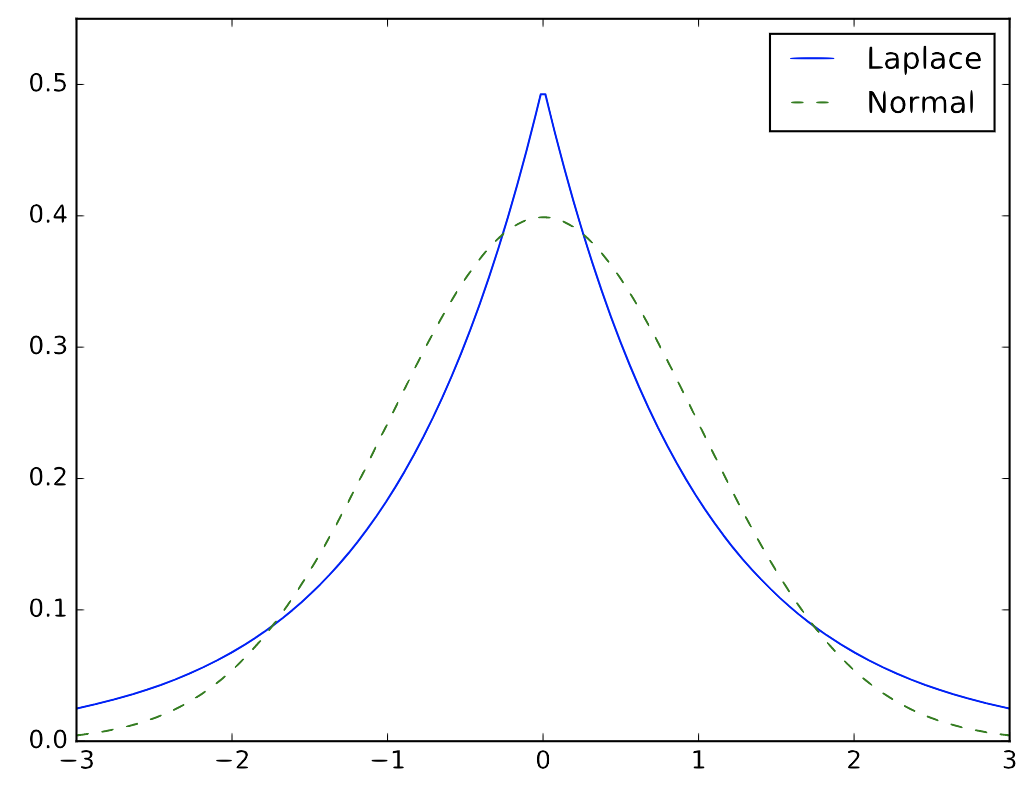
\includegraphics[width=.9\textwidth]{laplacen.png}
			\end{column}
			\begin{column}{.5\textwidth}
				$Pr(\eta = z) \sim$
			\end{column}
		\end{columns}
	
	Laplace noise has ``heavier tails'', meaning that it results in more outliers.
	
	\alert{This is a completely different justification for $\ell_1$ loss.}
\end{frame}

\begin{frame}
	\frametitle{bayesian regularization}
	\begin{center}
	\textbf{Recall goal is to maximize over $\vec{\beta}$:}
	\begin{align*}
		\Pr(\vec{\beta} \mid \bv{X},\vec{y} )  = \frac{\Pr(\bv{X},\vec{y} \mid  \vec{\beta} ) \Pr(\vec{\beta} )  }{\Pr(\bv{X},\vec{y} )}.
	\end{align*}
	\sout{assume all $\vec{\beta}$'s equally likely}	
	
	\textbf{Bayesian view:} Assume values in $\vec{\beta} = [\beta_1, \ldots, \beta_d]$ are generated from some probabilistic model. 
	\end{center}

\begin{itemize}
	\item \textbf{Common model:} Each $\beta_i$ drawn from $N(0,\gamma^2)$, i.e. normally distributed, independent.
	\item Encodes a belief that we are unlikely to see models with large coefficients. 
\end{itemize}
\end{frame}

\begin{frame}
	\frametitle{bayesian regularization}
	\textbf{Goal:}  choose $\vec{\beta}$ to maximize:
	\begin{align*}
		\Pr(\vec{\beta} \mid \bv{X},\vec{y} )  = \frac{\Pr(\bv{X},\vec{y} \mid  \vec{\beta} ) \Pr(\vec{\beta} )  }{\Pr(\bv{X},\vec{y} )} .
	\end{align*}
	\begin{itemize}
	\item We can still ignore the ``evidence'' term $\Pr(\bv{X},\vec{y})$ since it is a constant that does not depend on $\vec{\beta}$.
	\item $\Pr(\vec{\beta}) = \Pr({\beta}_1)\cdot  \Pr({\beta}_2)\cdot \ldots \cdot \Pr({\beta}_d)$
	\item $\Pr(\vec{\beta})  \sim $
	\end{itemize}
\end{frame}

\begin{frame}
	\frametitle{bayesian regularization}
	\begin{align*}
	\vec{\beta}* &=\argmax_{\vec{\beta}}\Pr(\bv{X},\vec{y} \mid  \vec{\beta} ) \cdot \Pr(\vec{\beta} ) \\
	& = \argmax_{\vec{\beta}} \prod_{i=1}^n e^{-(y_i - \langle \vec{x}_i, \vec{\beta} \rangle)^2/\sigma^2} \cdot \prod_{i=1}^n e^{-(\beta_i)^2/\gamma^2} \\ 
	&= \argmax_{\vec{\beta}}  \sum_{i=1}^n -(y_i - \langle \vec{x}_i, \vec{\beta} \rangle)^2/\sigma^2 + \sum_{i=1}^d -(\beta_i)^2/\gamma^2\\
	&= \argmin_{\vec{\beta}}  \sum_{i=1}^n (y_i - \langle \vec{x}_i, \vec{\beta} \rangle)^2+ \frac{\sigma^2 }{\gamma^2}\sum_{i=1}^d (\beta_i)^2/\sigma^2.
	\end{align*}
	
	Choose $\vec{\beta}*$ to minimize $\|\vec{y} - \bv{X}\vec{\beta}\|_2^2 + \frac{\sigma^2 }{\gamma^2}\|\vec{\beta}\|_2^2$.
	
	
	\alert{Completely different justification for ridge regularization!}
\end{frame}

\begin{frame}
	\frametitle{bayesian regularization}
	\textbf{Test your intuition:} What modeling assumption justifies LASSO regularization: $\min \|\vec{y} - \bv{X}\vec{\beta}\|_2^2 + \lambda\|\vec{\beta}\|_1$?
\end{frame}

\begin{frame}[standout]
	linear classification
\end{frame}

\begin{frame}
	\frametitle{motivating problem}
	\textbf{Breast Cancer Biopsy:} Determine if a breast lump in a patient is \emph{malignant} (cancerous) or \emph{benign} (safe). 
	\begin{itemize}
		\item Collect cells from lump using \emph{fine needle biopsy}.
		\item Stain and examine cells under microscope.
		\item Based on certain characteristics (shape, size, cohesion) determine if likely malignant or not).
	\end{itemize}
\begin{center}
	\includegraphics[width=.6\textwidth]{fna_labeled.png} \includegraphics[width=.4\textwidth]{cells.png}
\end{center}
\end{frame}

\begin{frame}
	\frametitle{motivating problem}
	\textbf{Demo:} \texttt{demo\_breast\_cancer.ipynb}
	
	\textbf{Data:} UCI machine learning repository
	\begin{center}
		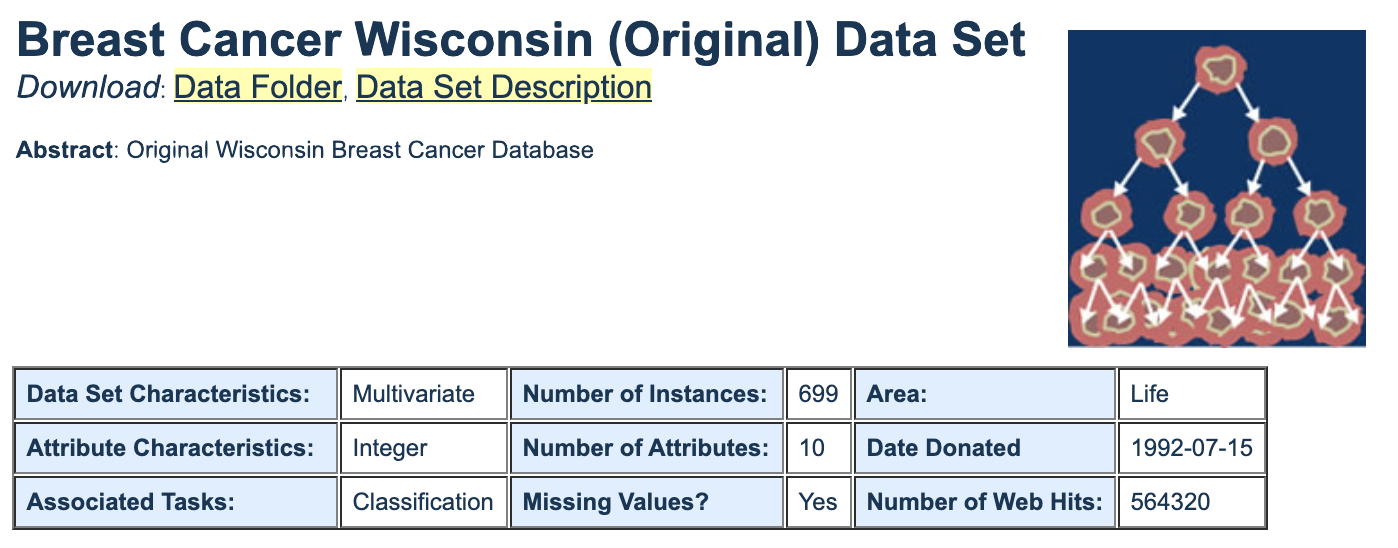
\includegraphics[width=.9\textwidth]{uci_cancer.png}
		
		\footnotesize{\url{https://archive.ics.uci.edu/ml/datasets/breast+cancer+wisconsin+(original)}}
	\end{center}

	\textbf{Features:} 10 numerical scores about cell characteristics (Clump Thickness, Uniformity, Marginal Adhesion, etc.)
	
\end{frame}

\begin{frame}
	\frametitle{motivating problem}
	\textbf{Data:} $(\vec{x}_1, y_1), \ldots, (\vec{x}_n, y_n)$. 
	
	$\vec{x}_i = [1,5,4\ldots, 2]$ contains score values. 
	
	Label $y_i\in \{0,1\}$ is $0$ if benign cells, $1$ if malignant cells.
	
	\textbf{Goal:} Based on scores (which would be collected manually, or even learned on their own using an ML algorithm) predict if a sample of cells is malignant or benign. 
	
	\textbf{Approach:}
	\begin{itemize}
		\item Naive Bayes Classifier can be extended to $\vec{x}$ with numerical values (instead of binary values as seen before).  Will see on homework.
		\item \textbf{Today:} Learn a different type of classifier.
	\end{itemize}
\end{frame}

\begin{frame}
	\frametitle{begin by plotting data}
	We pick two variables, \emph{Margin Adhesion} and \emph{Size Uniformity} and plot a scatter plot. Points with label 1 (malignant) are plotted in blue, those with label 2 (benign) are plotted in green.
	\begin{center}
		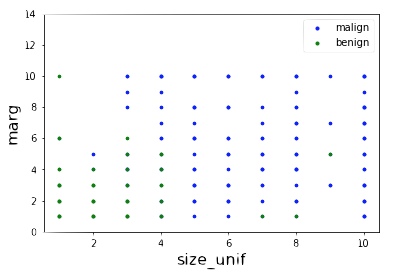
\includegraphics[width=.7\textwidth]{unjittered.png}
		
		\textbf{Lots of overlapping points! Hard to get a sense of the data.}
	\end{center}
\end{frame}

\begin{frame}
	\frametitle{plotting with jitter}
	\textbf{Simple + Useful Trick:} data \emph{jittering}. Add tiny random noise (using e.g. \texttt{np.random.randn}) to data to prevent overlap. 
	\begin{center}
		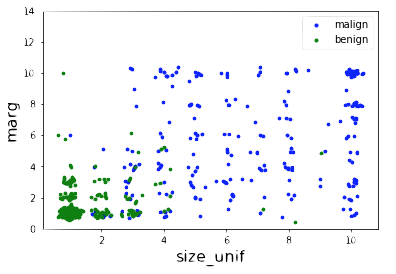
\includegraphics[width=.7\textwidth]{jittered.png}
		
		Noise is only for plotting. It is not added to the data for training, testing, etc. 
	\end{center}
\end{frame}

\begin{frame}
	\frametitle{brainstorming}
	\begin{center}
		Any ideas for possible \emph{classification rules} for this data?
		
		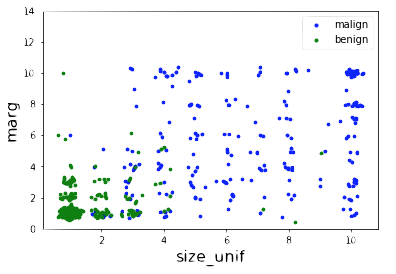
\includegraphics[width=.7\textwidth]{jittered.png}
		
	\end{center}
\end{frame}

\begin{frame}
	\frametitle{linear classifier}
	\begin{center}
		Given vector of predictors $\vec{x}_i \in \R^d$ (here $d = 2$) find a parameter vector $\vec{\beta} \in \R^d$ and threshold $\lambda$.
		\begin{itemize}
			\item Predict $y_i = 0$ if $\langle \vec{x}_i,\vec{\beta}\rangle \leq \lambda$.
			\item Predict $y_i = 1$ if $\langle \vec{x}_i,\vec{\beta}\rangle > \lambda$
		\end{itemize} 
		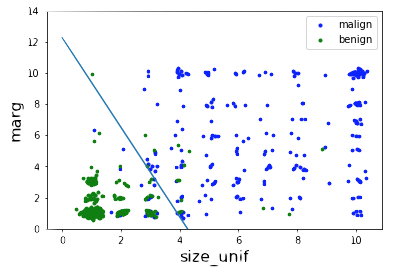
\includegraphics[width=.6\textwidth]{linear_classifier.png}
		
		\vspace{-.5em}
		Line has equation $\langle \vec{x},\vec{\beta}\rangle  = \lambda$. 
	\end{center}
\end{frame}

\begin{frame}
	\frametitle{linear classifier}
	\begin{center}
		As long as we append a $1$ onto each data vector $\vec{x}_i$ (i.e. a column of ones onto the data matrix $\bv{X}$) like we did for linear regression, an equivalent function is:
		\begin{itemize}
			\item Predict $y_i = 0$ if $\langle \vec{x}_i,\vec{\beta}\rangle \leq 0$.
			\item Predict $y_i = 1$ if $\langle \vec{x}_i,\vec{\beta}\rangle > 0$
		\end{itemize} 
		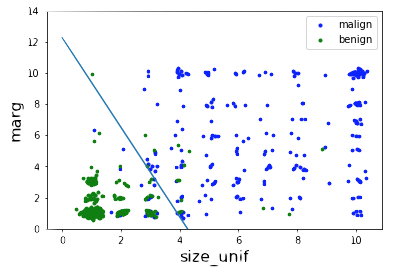
\includegraphics[width=.5\textwidth]{linear_classifier.png}
		
		\vspace{-.5em}
		Line has equation $\langle \vec{x},\vec{\beta}\rangle  = 0$. 
	\end{center}
\end{frame}

\begin{frame}
	\frametitle{$0-1$ loss}
	\textbf{Question:} How do we find a good linear classifier automatically?
	
	\textbf{Loss minimization approach (first attempt):}
	\begin{itemize}
		\item \textbf{Model}\footnote{$\mathbbm{1}[\text{event}]$ is the indicator function: it evaluates to 1 if the argument inside is true, 0 if false.}: 
		\begin{align*}
			f_{\vec{\beta}}(\vec{x}) = \mathbbm{1}\left[\langle \vec{x},\vec{\beta}\rangle > 0\right]
		\end{align*}
		\item \textbf{Loss function}: ``$0-1$ Loss''
		\begin{align*}
		L(\vec{\beta}) = \sum_{i=1}^n |f_{\vec{\beta}}(\vec{x}_i -y_i|
		\end{align*}
	\end{itemize}
\end{frame}

\begin{frame}
	\frametitle{$0-1$ loss}
	\textbf{Problem with $0-1$ loss:}
	\vspace{-.5em}
	\begin{center}
		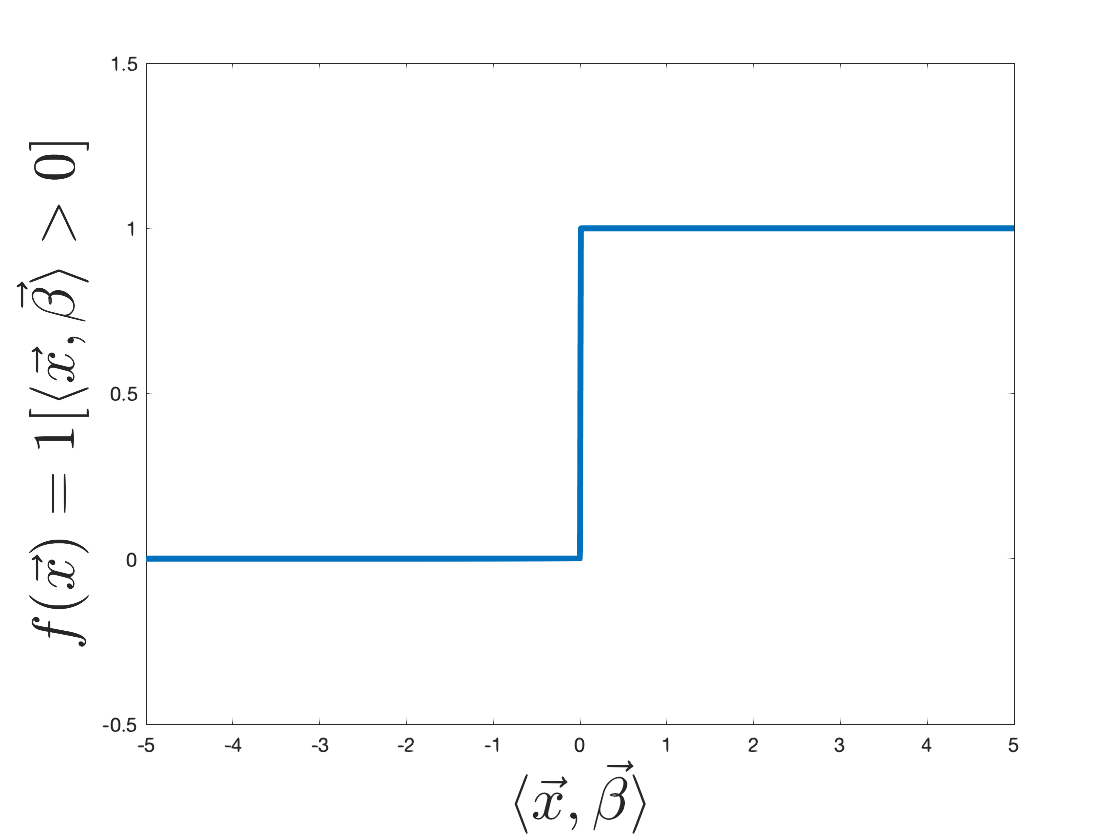
\includegraphics[width=.5\textwidth]{sharp_function.png}
			\vspace{-.5em}
	\end{center}
\begin{itemize}
	\item The loss function $L(\vec{\beta})$ is not differentiable because $f_{\vec{\beta}}(\vec{x})$ is discontinuous.
	\item Impossible to take the gradient, very hard to minimize loss to find optimal $\vec{\beta}$.
	\item Non-convex function (will make more sense next lecture).
\end{itemize}
\end{frame}

\begin{frame}
	\frametitle{linear classifier via square loss}
	\textbf{Question:} How do we find a good linear classifier automatically?
	
	\textbf{Loss minimization approach (second attempt):}
	\begin{itemize}
		\item \textbf{Model}: 
		\begin{align*}
		f_{\vec{\beta}}(\vec{x}) = \mathbbm{1}\left[\langle \vec{x},\vec{\beta}\rangle > 1/2\right]
		\end{align*}
		\item \textbf{Loss function}: ``Square Loss''
		\begin{align*}
		L(\vec{\beta}) = \sum_{i=1}^n (\langle \vec{x},\vec{\beta}\rangle-y_i)^2
		\end{align*}
	\end{itemize}
Intuitively tries to make $\langle \vec{x},\vec{\beta}\rangle$ close to 0 for examples in class 0, close too 1 for examples in class $1$. 
\end{frame}

\begin{frame}
	\frametitle{linear classifier via square loss}
	We can solve for $\vec{\beta}$ my just solving a least squares multiple linear regression problem.
	\begin{center}
		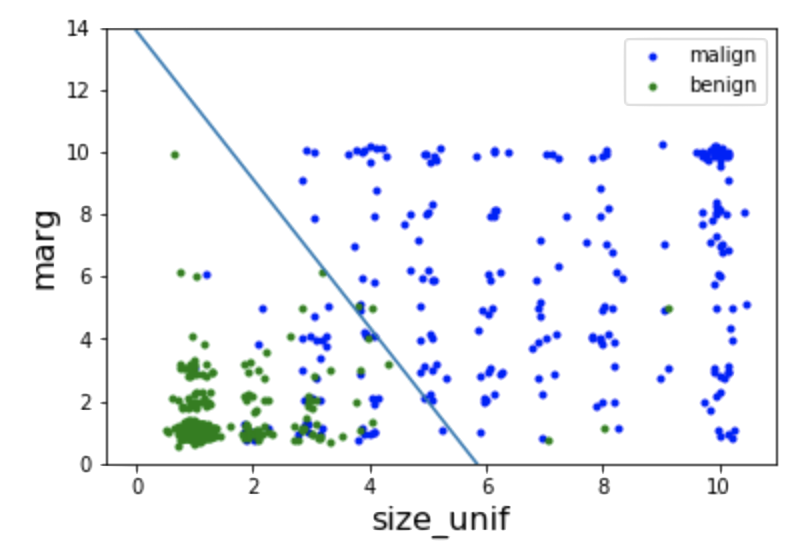
\includegraphics[width=.5\textwidth]{squareloss.png}
		\vspace{-.5em}
	\end{center}
	Do you see any issues here?
\end{frame}

\begin{frame}
	\frametitle{linear classifier via square loss}
	\textbf{Problem with square loss:}
	\vspace{-.5em}
	\begin{center}
		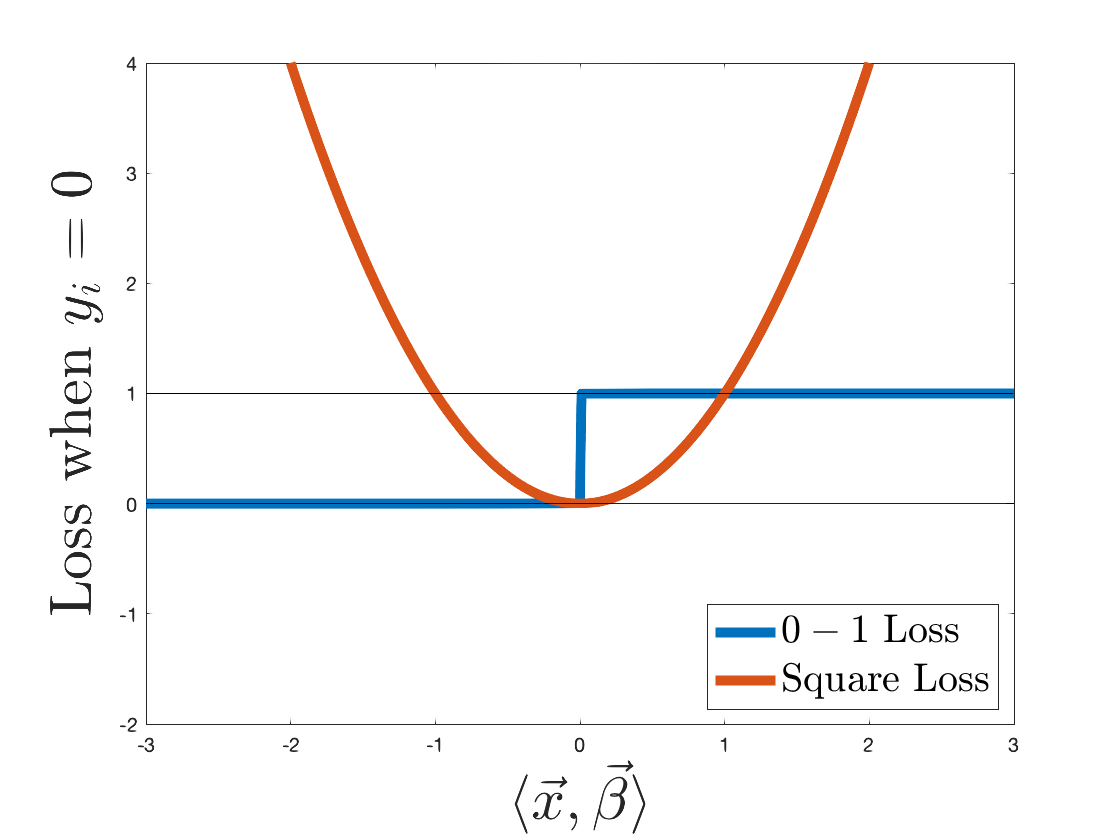
\includegraphics[width=.5\textwidth]{square_loss_compare.png}
		\vspace{-.5em}
	\end{center}
	\begin{itemize}
		\item Loss increases if $\langle \vec{x},\vec{\beta}\rangle > 1$ even if correct label is $1$. Or if $\langle \vec{x},\vec{\beta}\rangle < 0$ even if correct label is $0$.
		\item Intuitively we don't want to ``punish'' these cases.
	\end{itemize}
\end{frame}

\begin{frame}[t]
	\frametitle{logistic regression}
	Let $h_{\vec{\beta}}(\vec{x})$ be the \textbf{\alert{logistic function}}:
	\begin{align*}
		h_{\vec{\beta}}(\vec{x}) = \frac{1}{1 + e^{-\langle\vec{\beta},\vec{x}\rangle}}
	\end{align*}
\end{frame}

\begin{frame}[t]
	\frametitle{logistic regression}
	Let $h_{\vec{\beta}}(\vec{x})$ be the \textbf{\alert{logistic function}}:
	\begin{align*}
	h_{\vec{\beta}}(\vec{x}) = \frac{1}{1 + e^{-\langle\vec{\beta},\vec{x}\rangle}}
	\end{align*}
	\begin{center}
		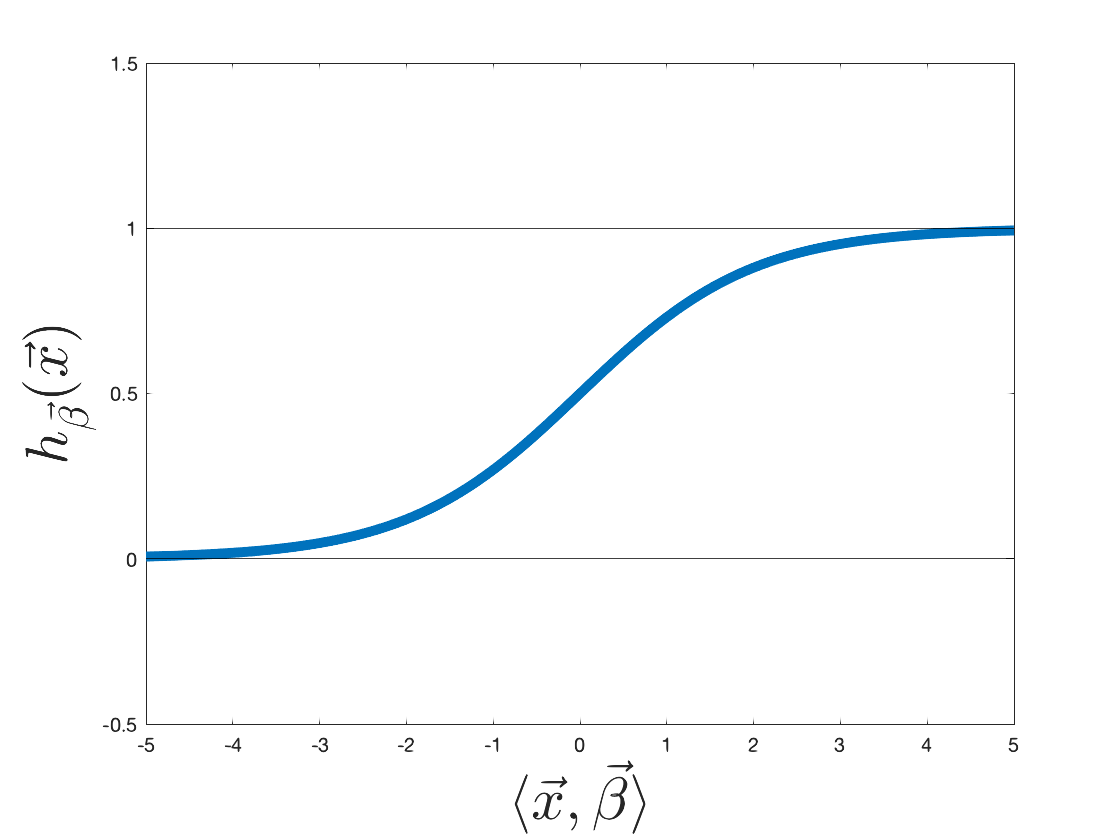
\includegraphics[width=.66\textwidth]{logistic_function.png}
	\end{center}
\end{frame}

\begin{frame}
	\frametitle{logistic regression}
	\textbf{Loss minimization approach (what works!):}
	\begin{itemize}
		\item \textbf{Model}: Let $h_{\vec{\beta}}(\vec{x}) = \frac{1}{1 + e^{-\langle\vec{\beta},\vec{x}\rangle}}$
		\begin{align*}
		f_{\vec{\beta}}(\vec{x}) = \mathbbm{1}\left[h_{\vec{\beta}}(\vec{x})  > 1/2\right]
		\end{align*}
		\item \textbf{Loss function}: ``Logistic loss'' aka ``Cross-entropy loss''
		\begin{align*}
		L(\vec{\beta}) = - \sum_{i=1}^n y_i \log(h_{\vec{\beta}}(\vec{x})) + (1-y_i) \log(1 - h_{\vec{\beta}}(\vec{x})) 
		\end{align*}
	\end{itemize}
\vspace{1em}

\end{frame}

\begin{frame}
	\frametitle{logistic loss}
	\textbf{Logistic Loss:} $L(\vec{\beta}) = - \sum_{i=1}^n y_i \log(h_{\vec{\beta}}(\vec{x})) + (1-y_i) \log(1 - h_{\vec{\beta}}(\vec{x})) $
	\vspace{-.5em}
	\begin{center}
		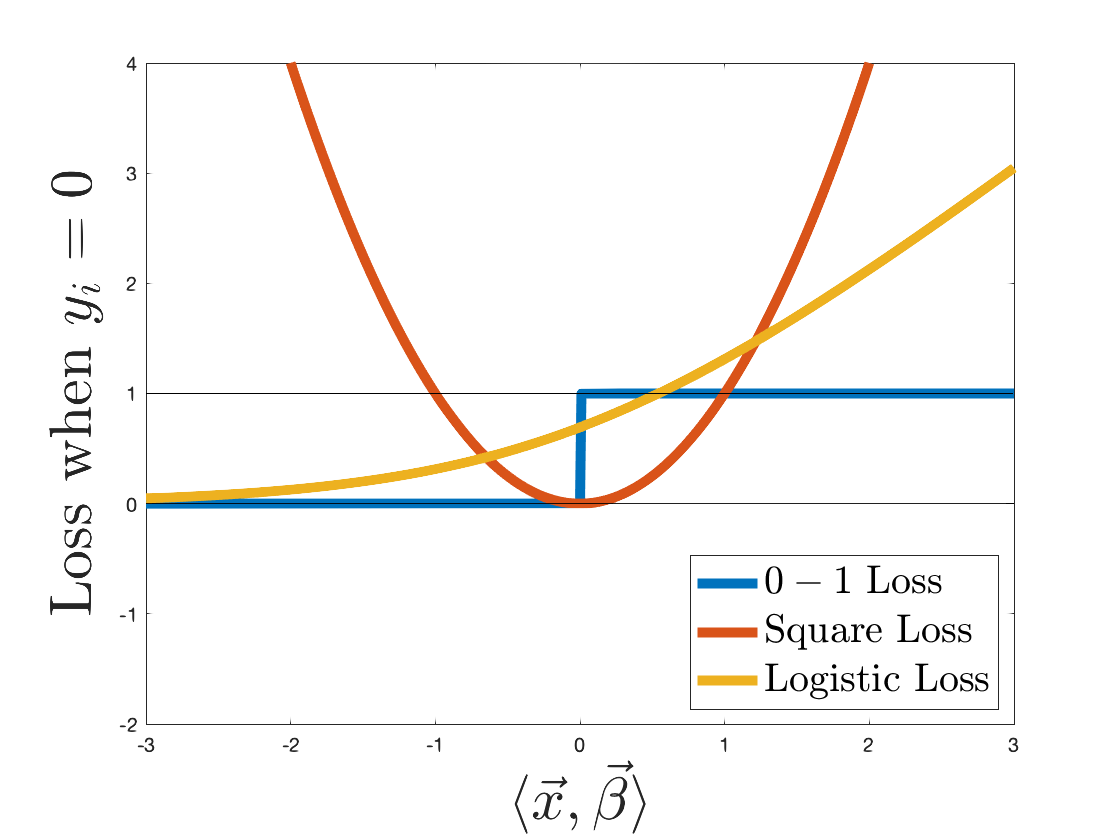
\includegraphics[width=.6\textwidth]{all_loss.png}
	\end{center}

\end{frame}

\begin{frame}
	\frametitle{logistic loss}
	\begin{itemize}
		\item Convex function, can be minimized using gradient descent (next lecture).
		\item Works well in practice.
		\item Good Bayesian motivation: see posted lecture notes if you are interested.
	\end{itemize}
\begin{center}
	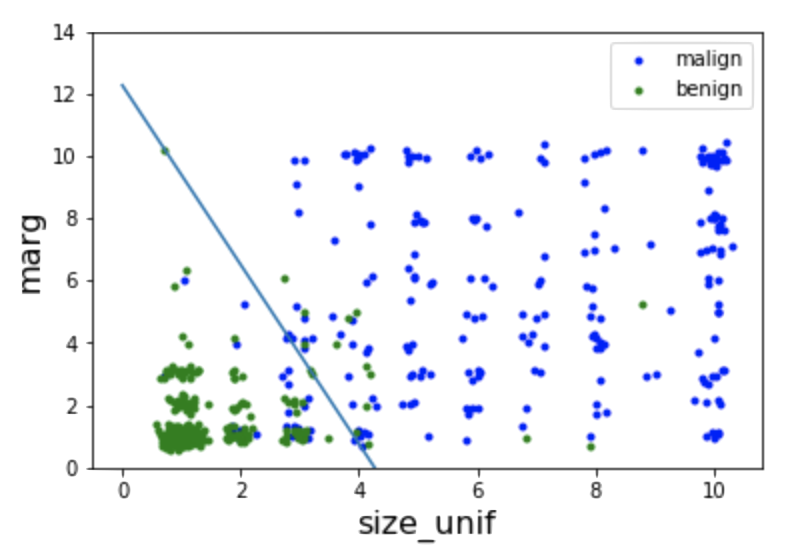
\includegraphics[width=.5\textwidth]{logisticloss.png}
	
	\textbf{Fit using logistic regression/log loss.}
\end{center}
\end{frame}

\begin{frame}
	\frametitle{error in classification}
	Once we have a classification algorithm, how do we judge its performance?
	\begin{itemize}
		\item \textbf{Simplest answer:} Error rate = fraction of data examples misclassified in test set.
		\item What are some issues with this approach?
	\end{itemize}
\end{frame}

\begin{frame}
	\frametitle{error in classification}
	\begin{columns}
		\begin{column}{.5\textwidth}
			\begin{itemize}
				\item \textbf{Precision:} Fraction of positively labeled examples (label 1) which are correct.
				\item \textbf{Recall:} Fraction of true positives that we labeled correctly with label 1.
			\end{itemize}
		
		\vspace{1em}
		\textbf{Question:} Which should we optimize for medical diagnosis?
		\end{column}
		\begin{column}{.5\textwidth}
			\vspace{1em}
			
			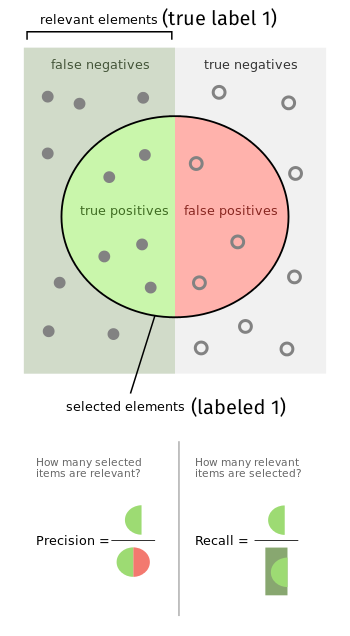
\includegraphics[width=.8\textwidth]{precision_recall.png}
		\end{column}
	\end{columns}
\end{frame}


\begin{frame}
	\frametitle{error in classification}
	\textbf{Logistic regression workflow:}
	\begin{itemize}
		\item Select $\vec{\beta}$ via training and compute $h_{\vec{\beta}}(\vec{x}_i) = \frac{1}{1 + e^{-\langle\vec{x}_i,\vec{\beta}\rangle}}$ for all $\vec{x}_i$.
		\item Predict $y_i = 0$ if  $h_{\vec{\beta}}(\vec{x}_i)  \leq \lambda$, $y_i = 1$ if  $h_{\vec{\beta}}(\vec{x}_i)  > \lambda$.
		\item Default value of $\lambda$ is $1/2$. Increasing $\lambda$ improves \emph{precision}. Decreasing $\lambda$ improves \emph{recall}.
	\end{itemize}
\end{frame}




\end{document} 








